% \PP{Adversarial Attacks Analysis} We discussed robustness to mimicry attacks in Section~\ref{sec:mimicry}. Here, we address vulnerabilities to other types of adversarial attacks, including gradient-based attacks, model poisoning, and inference attacks (discussed in Section~\ref{sec:privacy}). Addressing these attacks is beyond the scope of this paper, as we focus on establishing an end-to-end framework for privacy-aware PIDS. We plan to integrate advancements in adversarial defense mechanisms against such attacks into \Sys to enhance its robustness in future work. These integrations are discussed below.

% Gradient-based adversarial attacks~\cite{chakraborty2021survey} typically require white-box access to the target machine learning model, including its parameters. This necessity often renders them impractical for real-world applications. In contrast, black-box attacks, which utilize iterative, query-based techniques, tend to be more detectable and complex to implement due to their conspicuous nature. Such attacks are feasible if an attacker manages to compromise a client machine. However, during the operational phase, a compromised client cannot affect other clients because they are working independently. Several existing defenses can be employed during model training to enhance the system's resilience against these attacks. Adversarial training~\cite{tramer2019adversarial} is one effective strategy, wherein the model is trained with perturbed input data to increase its robustness to such attacks.

% During the training phase, poisoning attacks executed by malicious actors may introduce corrupt weights to compromise the global model~\cite{jagielski2018manipulating}. To improve \Sys's resilience against such threats, several defensive methods can be used. Among these, advanced model aggregation methods, such as Multi-Krum~\cite{munoz2019byzantine}, can be particularly effective. This method employs clustering techniques on the central server to identify anomalous updates during model aggregation. Consequently, outlier updates are removed, enhancing the system's robustness against poisoning.

\section{Adversarial Attacks Analysis}
\label{sec:adversarial}

\begin{figure}[!t]
  \centering
  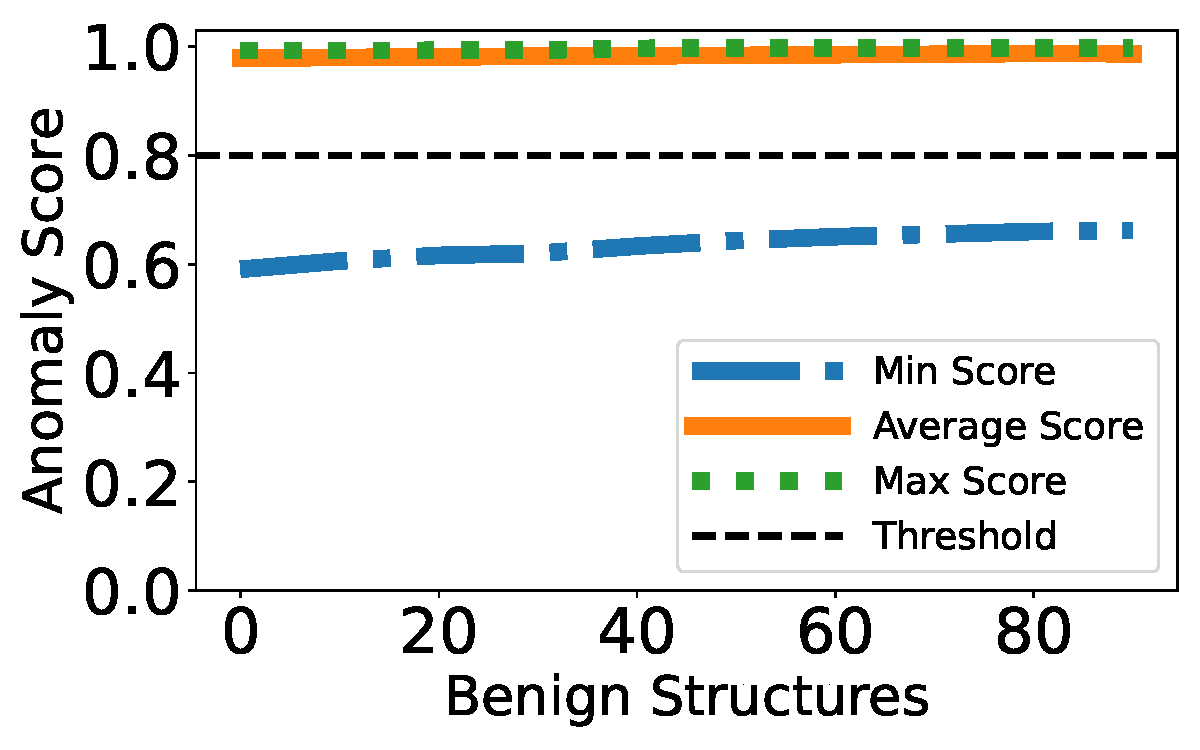
\includegraphics[width=0.34\textwidth]{fig/adversarial.pdf}
  \caption{Adversarial mimicry attack analysis.}
  \label{mimicryattack}
  \vspace{-2ex}
\end{figure}


In this section, we analyze the robustness of our system against mimicry, model poisoning, and gradient-based attacks. Membership inference attacks are discussed in Section~\ref{sec:privacy}.

\PP{Mimicry Attacks}  We evaluated our system's resilience against the adversarial mimicry attack detailed by Goyal et al.~\cite{goyal2023sometimes} and compared its robustness with \flash. The attack aims to mimic benign graph embeddings, integrating benign node structures to evade detection. Using the E3 dataset, similar to \flash for fair comparison, our findings (shown in Figure~\ref{mimicryattack}) reveal that our detector remains robust; the integration of benign structures has a minimal impact on anomaly scores. Our system's superior robustness is due to our process-categorization-based ensemble \gnnshort architecture, which allows model specialization for different system entities, enhancing detection of structural changes. Conversely, \flash, relying on a generalized model for anomaly detection, exhibits vulnerabilities to mimicry attacks, as it may miss critical details. As demonstrated by the authors, \flash initially experiences a drop in anomaly scores, increasing the likelihood of attack nodes evading detection—a vulnerability not present in our system. \footnote{PROVNINJA~\cite{mukherjee2023evading} is another mimicry attack that uses benign process profiles to find adversarial evasion strategies. It faces challenges against \pids like \flash and \Sys due to their multimodal architecture, which combines \wordvec for featurization and \gnnshort for anomaly detection. This complexity makes it difficult for attackers to create effective evasion strategies without accessing \wordvec directly or excessively querying the model, which conflicts with the black box nature of the assumed threat model of PROVNINJA.}



\PP{Model Poisoning Attacks} These occur when one or more malicious clients submit corrupted local model updates to the central server during training, thereby degrading the model’s performance. Existing methods typically assume an attack-free training phase, providing no defense against such attacks. We conducted experiments on the \optc dataset to assess the impact of poisoning attacks on our system, and we also evaluated how robust aggregation methods—such as Multi-Krum~\cite{munoz2019byzantine}—can enhance resilience.

Multi-Krum compares each client’s gradient with those of other clients, retaining only the most consistent updates. Since malicious updates must deviate significantly from benign ones to degrade performance, Multi-Krum effectively identifies and discards them as outliers. Figure~\ref{fig:poison} shows our experimental results using both FedAvg and Multi-Krum. With simple federated averaging, malicious noise critically affects the model by disrupting the benign distribution it learns. In contrast, Multi-Krum isolates and removes erroneous updates from malicious clients, preserving the global model. Notably, Multi-Krum assumes that fewer than one-third of all clients are malicious; therefore, in our experiments, we tested with a maximum of 30\% compromised clients.

\begin{figure}[!t]
    \centering
    \subfloat[FedAvg aggregation.]{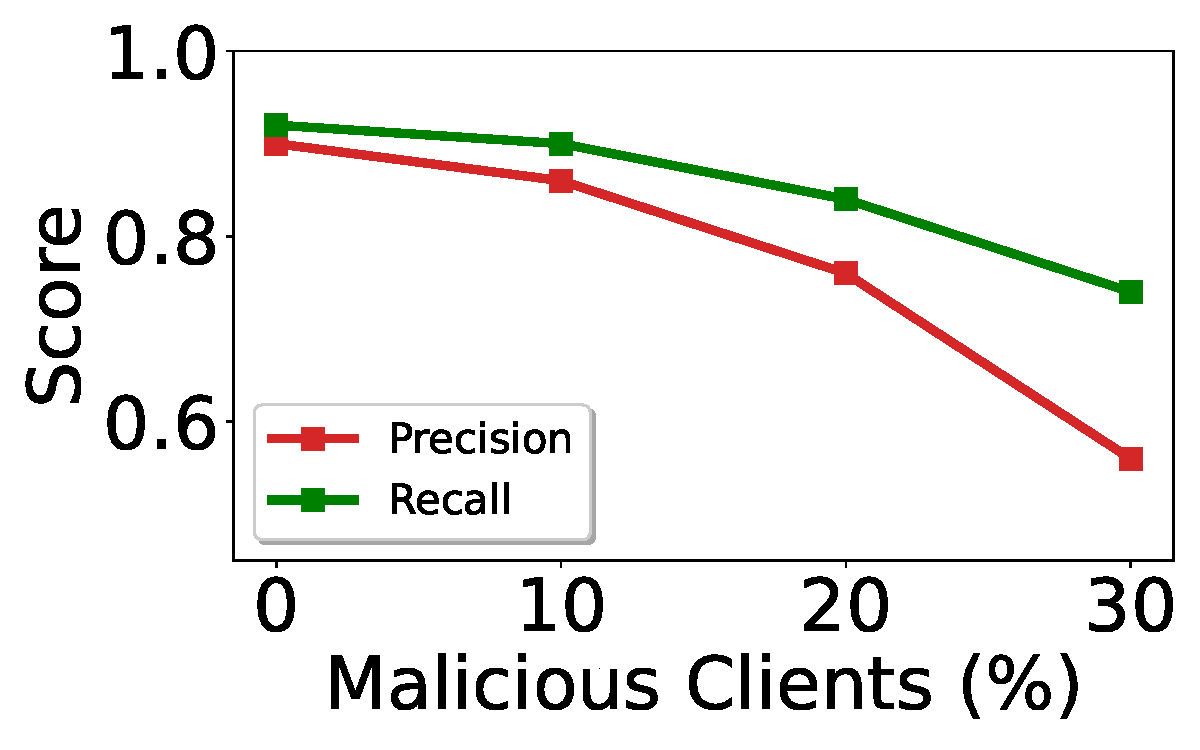
\includegraphics[width=0.23\textwidth]{fig/FedAvg_poisoning.pdf}\label{fedavgpoison}}
    \hfill
    \subfloat[Multi-Krum aggregation ]{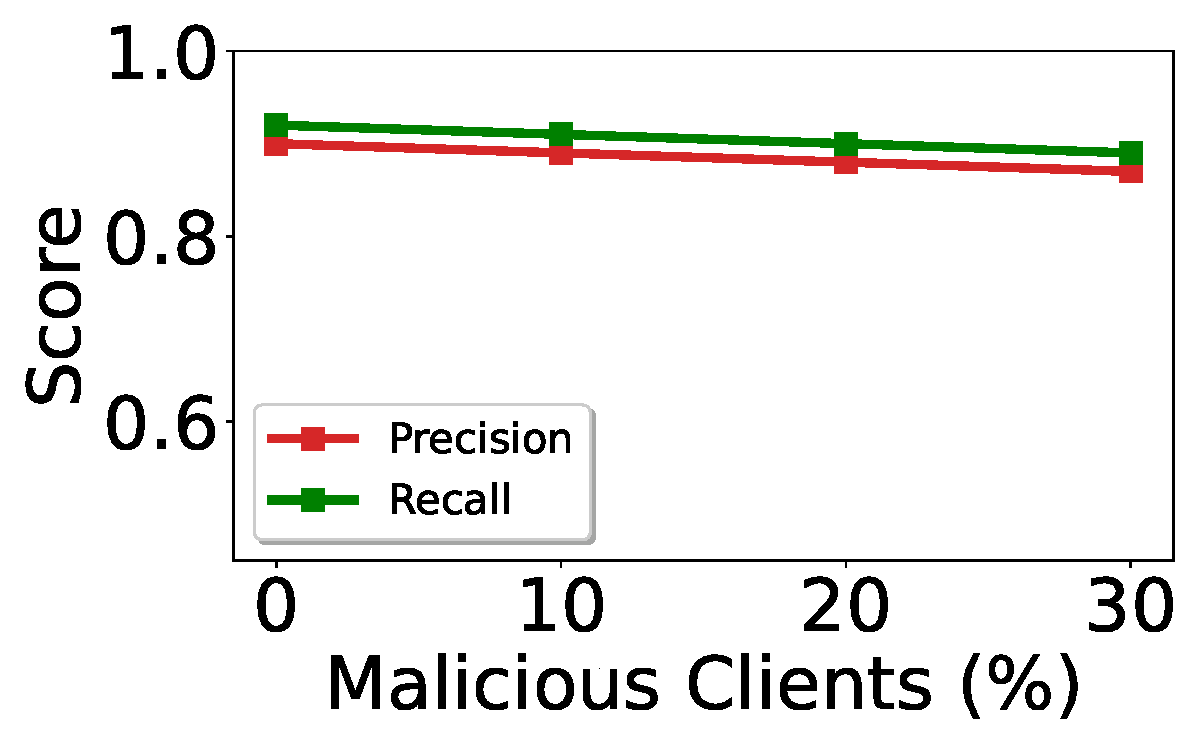
\includegraphics[width=0.23\textwidth]{fig/multi-krum.pdf}\label{multikrumpoison}}
    \hfill
    \caption{Model poisoning attack analysis.}
    \label{fig:poison}
    \vspace{-3ex}
  \end{figure}

\PP{Gradient-based Attacks} These attacks~\cite{chakraborty2021survey} exploit detailed knowledge of the target model, including its architecture and parameters, to calculate and apply malicious perturbations. Such white-box access allows an attacker to compute precise gradients that indicate how inputs should be modified to degrade the model’s performance. Other attacks tend to be black-box in nature, relying on iterative, query-based techniques to influence the model’s decisions. However, these repeated computations and queries run counter to the attacker’s aim of remaining inconspicuous, as they generate substantial activity and leave a significant footprint. Consequently, such attacks are often impractical in real-world scenarios. Several defenses can be employed during model training to bolster the system’s resilience against these threats. Adversarial training~\cite{tramer2019adversarial} is one effective strategy in which the model is trained on perturbed input data, thereby increasing its robustness against these attacks.

\subsection{Effect of differential privacy on accuracy}
\label{app:dp}

In Section~\ref{sec:privacy}, we analyze how our system design offers strong guarantees against model inference attacks. Here we discuss another alternative technique for preserving privacy through the use of Differential Privacy (DP). It can be integrated with federated learning to protect against inference attacks~\cite{lyu2020threats,nasr2019comprehensive,zari2021efficient}, though it comes at the cost of detection accuracy.

Differential privacy safeguards the model by injecting a controlled amount of Gaussian noise into its parameters, thereby concealing the influence of any individual data point. In our work, we adopt a node-level DP strategy, which ensures that each node’s features and labels are protected when noise is added to the gradient updates. As a result, individual node contributions remain obscured in the aggregated model parameters, reducing the likelihood of identifying specific nodes or their features. We conduct experiments to examine how varying levels of differential privacy noise affect the detection performance of \Sys. The noise is adjusted based on a privacy budget defined by~$\epsilon$. This noise is applied to local \gnnshort model updates before they are aggregated at the central server during federated averaging, as described in Section~\ref{sec:methodology}.

\begin{figure}[!t]
  \centering
  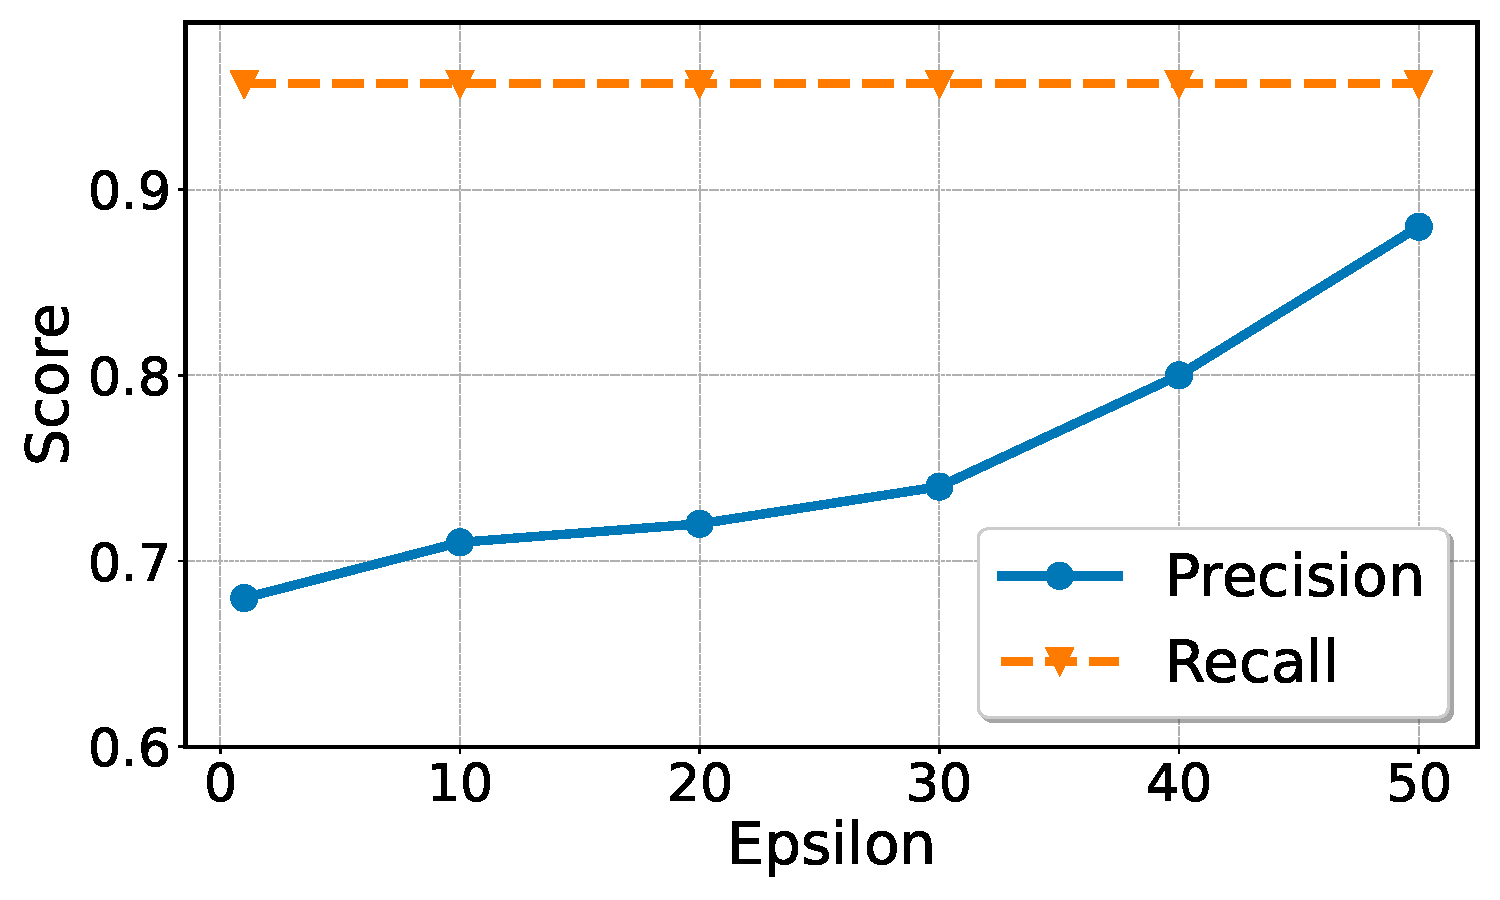
\includegraphics[width=0.3\textwidth]{fig/epsvsscore.pdf}
  \caption{Effect of differential privacy noise on detection using E3 dataset. Note that we observed similar results on the other datasets.}
  \label{epsvsscore}
  \vspace{-2ex}
\end{figure}


The privacy budget~$\epsilon$ plays a pivotal role. Lower values of $\epsilon$ increase the noise injected into the model, which enhances privacy at the expense of detection performance. Conversely, higher values of $\epsilon$ inject less noise, improving detection accuracy but offering weaker privacy guarantees. By tuning $\epsilon$ during training, we explore the balance between privacy and detection effectiveness across various settings. As shown in Figure~\ref{epsvsscore}, increasing the noise level (i.e., reducing $\epsilon$) degrades the model’s utility, thereby providing more privacy at the cost of lower accuracy.

Hence, although DP is a valid solution for protecting privacy, the accuracy deterioration that comes with it reduces its utility in the domain of intrusion detection, where high detection performance is needed. Due to these reasons, we do not use DP in \Sys and instead design a dual-server architecture to offer privacy guarantees without adding noise to the model updates.
